% \documentclass[amsmath,amssymb,twocolumn]{revtex4-2} 
\documentclass[%
 aip,
% jmp,
% bmf,
% sd,
% rsi,
 amsmath,amssymb,
%preprint,%
 reprint,%
%author-year,%
%author-numerical,%
% Conference Proceedings
]{revtex4-1}
\usepackage[utf8]{inputenc}
\usepackage[T1]{fontenc}
\usepackage[]{graphicx}
\usepackage{grffile}
\usepackage{longtable}
\usepackage{natbib}
\usepackage{wrapfig}
\usepackage{rotating}
\usepackage{amsmath,bm}
\usepackage{textcomp}
\usepackage{amssymb}
\usepackage{capt-of}
\usepackage{hyperref}
\usepackage[margin=1in]{geometry}
\usepackage{ulem}
\usepackage{xcolor}
\usepackage{float}


\newcommand{\lh}[1]{{\color{blue}{#1}}}
\newcommand{\jd}[1]{{\color{red}{#1}}}
\newcommand{\sj}[1]{{\color{magenta}{#1}}}

\begin{document}

\title{Hybrid physics-based and data-driven approach for molecular docking}

%\title{Exploring Energy Landscapes with thermodynamic mappings}


\author{Lukas Herron}

\affiliation{Biophysics Program and Institute for Physical Science and Technology, University of Maryland, College Park, MD, 20742, USA}
\affiliation{Institute for Health Computing, University of Maryland, Bethesda 20852, USA.}
\author{Jumana Dakka}
\affiliation{Schrodinger Inc., New York, NY, 10108, USA}
\author{Steven V. Jerome}
\affiliation{Schrodinger Inc., New York, NY, 10108, USA}



\begin{abstract}
Abstract TBD
\end{abstract}

\maketitle

\section{Introduction}

Structure-based drug discovery is an approach to precision medicine that aims to design small molecules that bind to protein targets with high specificity and affinity to alter their function \cite{drug-discovery-review}. Computational approaches have proven indispensable for reducing the vast space of possible small molecules to a small number of potentially high-affinity binders. Historically, the most successful computational strategies have been physics-based models that explicitly account for energetic\cite{trott2010autodock,verdonk2003gold,friesner2004glide} and entropic\cite{murphy2016wscore} contributions to the binding free energy. 

In recent years alternative approaches rooted in deep learning have emerged, all of which share a core assumption that the relevant interactions are represented in structural data and can be implicitly modeled by a neural network. In a landmark application of deep learning to biology and chemistry, AlphaFold2 (AF2) modeled protein structures to unprecedented accuracy by training an artificial intelligence system on coevolutionary information and the structural contents of the Protein Data Bank (PDB)\cite{jumper2021af2}. Since AF2 there has been an explosion of deep learning methods for predicting structures arising from molecular interactions\cite{krishna2024rfaa,abramson2024af3}, including ones specifically focused on molecular docking \cite{corso2022diffdock,qiao2024neuralplexer}. 

However, comparative studies find that, at present, classical docking methods significantly outperform deep learning ones. Deep learning methods struggle to predict binding poses for receptors from families outside the training data\cite{buttenschoen2024posebusters} and fail to model the molecular interactions that stabilize binding\cite{errington2024plif}, indicating that the amount and diversity of currently available training data is insufficient to learn physical chemistry {\it ab intio}.

Deep learning takes a fundamentally opposite approach to the physical sciences, using models with many more free parameters than are necessary to capture the underlying latent variables. A promising path for improving the generalizability of deep learning for science is to build inductive biases into models \cite{behler2007neuralnetworkpotentials,fuchs2020equivariance,musaelian2023allegro}, simultaneously decreasing the number of free parameters, improving data economy by constraining the solution space of the model, and improving generalization by incorporating relevant prior knowledge.

Among deep learning approaches to molecular docking, those based on diffusion models are particularly promising for introducing physical inductive biases. It has been shown that such biases may be introduced by, for example, defining equivariant diffusion dynamics\cite{hoogeboom2022equivariant}, restricting the diffusion to a manifold\cite{jing2022torsional,de2022riemannian}, or biasing the generative dynamics\cite{corso2023particle}. 



In this work, we present a hybrid physics-based and deep learning approach to molecular docking. We use DiffDock\cite{corso2022diffdock} -- a diffusion model -- to sample putative binding poses, then score and refine the poses with Glide\cite{friesner2004glide} -- a physics-based molecular docking algorithm. We further introduce the location of the binding site as an inductive bias by confining the generative dynamics with a biasing potential in a manner that introduces little computational overhead and does not require retraining the model.

We benchmark DiffDock-Glide on the Posebusters dataset, demonstrating improved generalization to novel sequences and recovery of crystal-like binding poses compared to DiffDock alone. We also virtual screen small molecules from the DUDE\cite{mysinger2012dude} dataset against AF2-generated receptor structures, showing enrichment that surpasses Glide alone.

\section{Method}


The hybrid molecular docking model is divided into two stages. The first stage involves generating a set of potential binding poses using DiffDock equipped with a modified generative process that optionally restricts generation to a putative binding site. The second stage involves refining and scoring the generated poses using Glide -- an industry leading physics-based molecular docking algorithm. We test the conditional DiffDock-Glide model using targets from the DUDE dataset, a dataset widely used for benchmarking virtual screening methods. DUDE provides known actives (binders) and challenging decoys (non-binders) for 102 targets across a diverse set of protein classes. In this benchmark we selected the same targets as those in Zhang et. al.\citep{zhang2023benchmarking}

\subsection{Binding site-conditional DiffDock}

DiffDock is a diffusion model that predicts binding poses for a small-molecule given its chemical identity and a target protein structure. It is also a {\it blind} docking algorithm -- anywhere inside or on the target protein's surface is a potential binding site. Still, in a realistic structure-based drug discovery campaign, one oftentimes knows the location of the binding site and would like to explore poses therein. To this end, we bias DiffDock's generative process towards the location of the site under the particle guidance framework\cite{corso2023particle}. We will briefly summarize the core operating principles of DiffDock before introducing the biasing mechanism.


% In structure-based drug design,  one often knows the location of the binding site and would like to explore poses therein. 


DiffDock incorporates internal symmetries of molecular conformers as
inductive biases. In the diffusion process, perturbations to molecular degrees of freedom are represented as a product space $\mathbb{P}$ of groups: $\mathbb{T}(3) \times SO(3) \times SO(2)^m$; $\mathbb{T}(3)$ is the group of 3D-translations; $SO(3)$ is 3D-rotations; $SO(2)^m$ are 2D-rotations of $m$ torsion angles. Clearly, the actions of $\mathbb{P}$ on a particular conformer will result in new conformers; it is then natural to ask if arbitrary conformers are connected through an action of $\mathbb{P}$. Indeed, Corso et. al.\cite{corso2022diffdock} show that any {\it typical}\footnote{An atypical conformer has all atoms collinear about an axis of rotation\cite{corso2022diffdock}} pair of conformers lie on a manifold $\mathcal{M}_\mathbf{c}$ defined by actions of $\mathbb{P}$, and further show that the groups factoring $\mathbb{P}$ act orthogonally.


DiffDock is a score-based diffusion model\cite{song2020sgm} -- that is, a {\it stochastic differential equation} (SDE) -- with dynamics on $\mathcal{M}_\mathbf{c}$:
\begin{equation}
    \begin{aligned}
    \label{eq:diffdock-sde}
        \mathrm{d}\mathbf{x} = - \lambda(\tau) 
        \left[ \mathbf{x} - \sigma^{\mathbb{P}}\mathbf{s}^\mathbb{P}_\theta(\mathbf{x}, \mathbf{y}, \tau) \right]
        \mathrm{d}\tau \\+ \sqrt{2 \lambda(\tau) \sigma^{\mathbb{P}}}\mathrm{d}\mathbf{B}^{\mathbb{P}}_\tau,
    \end{aligned}
\end{equation}
where $\mathbf{B}_\tau^{\mathbb{P}}$ is Brownian motion on $\mathcal{M}_{\mathbf{c}}$, $\lambda(\tau)$ is a time dilation factor to accelerate convergence, and $\sigma^{\mathbb{P}}$ is the scale of the noise perturbations. The vectors $\mathbf{x}$ and $\mathbf{y}$ -- containing the positions of the ligand and protein backbone atoms respectively -- are inputs to a score network $\mathbf{s}_\theta$. The score network acts as a time-dependent vector field on $\mathcal{M}_{\mathbf{c}}$ that generates binding poses from noise vectors by simulating Eq. \ref{eq:diffdock-sde} from $\tau = 0$ to $\tau = 1$.

We condition Eq. \ref{eq:diffdock-sde} on a putative binding site by biasing the translational diffusion:
\begin{equation}
    \label{eq:diffdock-sde-conditional}
        \mathbf{s}^{\mathbb{T}(3)}_\theta(\mathbf{x}, \mathbf{y}, \tau)\rightarrow \mathbf{s}^{\mathbb{T}(3)}_\theta(\mathbf{x}, \mathbf{y}, \tau) - \gamma \nabla \Phi(\mathbf{r},\mathbf{r}_0)
\end{equation}
with $\Phi$ -- a potential with gradient
\begin{equation}
    \begin{aligned}
    \nabla_{r_i}&\Phi(\mathbf{r}, \mathbf{r}_0) = \\
    &\begin{cases} 
    0 & \text{if } d_i \leq r_{\mathrm{min}} \\
    (d_i(\mathbf{r}, \mathbf{r}_{0}) - r_{\mathrm{min}})^2 & \text{if } r_{\mathrm{min}} < d_i < r_{\mathrm{max}} \\
    (r_{\mathrm{max}} - r_{\mathrm{min}})^2 & \text{if } d_i \geq r_{\mathrm{max}}.
    \end{cases}
    \end{aligned}
\end{equation}

$\Phi(\mathbf{r}, \mathbf{r}_0)$ characterizes the geometry and location binding site: $\mathbf{r}_0$ is the center of the site, $r_{\mathrm{min}}$ is the radius, and $r_{\mathrm{max}}$ limits the gradient for numerical stability. The function $d_i$ measures the distance between the $i-$th component of $\mathbf{r}$ and $\mathbf{r}_0$, and the parameter $\gamma$ controls the strength of the potential. When $\gamma=0$ the generative process in Eq. \ref{eq:diffdock-sde}, is {\it unconditional}, i.e. the center of mass $\mathbf{r}$ freely explores the entire protein surface; in contrast, when $\gamma > 0$, the generative process is {\it conditional} and the center of mass is biased by $\Phi$ towards a spherical region of radius $r_\mathrm{min}$ centered around $\mathbf{r}_0$.

\subsection{DiffDock--Glide}
DiffDock produces a set of putative binding poses that are ranked by a second neural network -- a confidence model trained on the same dataset as DiffDock. The role of the confidence model is analogous to that of an energy function in a physics-based docking algorithm. However, unlike scoring functions based on physics and chemistry, the confidence model is not interpretable since the contributing factors are entangled.

Specifically, Buttenschoen et. al.\cite{buttenschoen2024posebusters} demonstrate that DiffDock-generated poses exhibit significant imperfections and fail to meet PoseBuster's valid pose criteria. This discrepancy arises because deep learning methods often lack several key aspects of molecular mechanics force fields, which are crucial for accurate docking.

Instead, we use Glide's post-docking minimization (PDM) pipeline to refine the generated poses. PDM runs an energy minimization step that adjusts the positions of the ligand atoms in the field of the receptor using rigid-body translations and rotations and reorienting the end-group rotatable bonds using torsional alterations. Glide then assigns a score to all poses based on the energy minimization terms derived from PDM. The score is empirically parameterized to approximate the binding free energy $\Delta$G of a ligand by rewarding or penalizing interactions such as van der Waals hydrophobic interactions, electrostatic Coulomb interactions and internal strain energy \cite{friesner2004glide}. 

Since Glide explicitly models the physical chemistry of small-molecule interactions it is expected to generalize well outside of DiffDock's training distribution. We refine DiffDock-generated poses using Glide's minimization model to optimize their orientation within the binding pocket. The resulting lower-energy conformations of the ligand-protein complexes are then ranked using Glide's scoring function.

\begin{figure*}[ht!]%
   \centering
   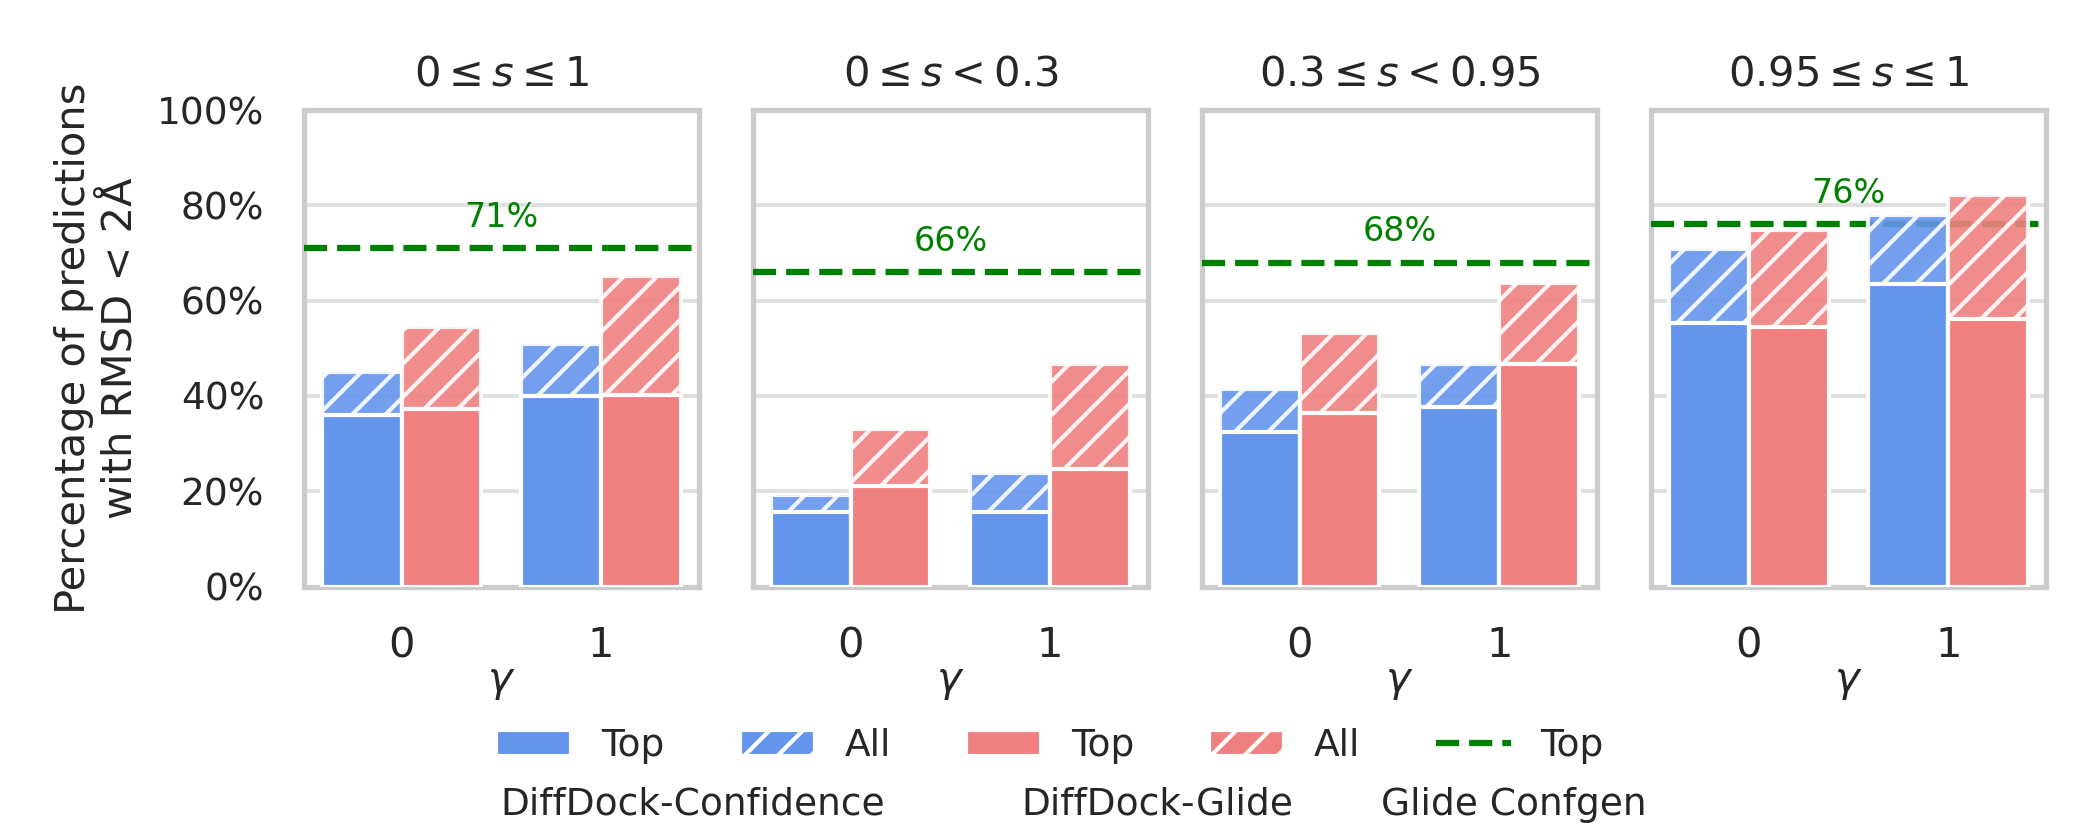
\includegraphics[
   width=\textwidth
   ]{pb_results.png}
   \caption{{\bf Performance of DiffDock-Glide on the PoseBusters dataset.} The percentage of PoseBusters (PB) systems that have an RMSD within 2{\AA} of the crystal pose is presented for five selection criteria across three values of $\gamma$. Glide Confgen (red line) presented as a baseline. The leftmost panel summarizes performance for the entire PB dataset, and the remaining panels stratify the PB dataset by sequence similarity ($s$) to PDBBind General Set v2020. Hatched bars denote poses selected prior to minimization, while solid bars indicate poses selected post-minimization.}
   \label{fig:pb-result}%
\end{figure*}

\section{Applications}
\label{sec:applications}

We explore two applications of the hybrid DiffDock--Glide model: molecular docking and virtual screening. 

\begin{itemize}
    \item Section \ref{sec:molecular-docking} explores the ability of DiffDock-Glide to dock small molecules against receptors in the PoseBusters dataset. Our results indicate that binding site conditioning and energy minimization improve generalization to receptors outside the training set and increase the fraction of systems for which a pose less than 2{\AA} in root mean squared deviation (RMSD) from the crystal pose is sampled.
    
    \item Section \ref{sec:virtual-screening} explores the ability of DiffDock-Glide to provide enrichment in small molecule virtual screens. We screen small molecules in the DUDE dataset against receptor structures generated by AF2 and obtain enrichments broadly surpassing those obtained from Glide alone.

\end{itemize}

\subsection{Molecular Docking}
\label{sec:molecular-docking}



Molecular docking aims to predict the binding pose of a small molecule with a receptor target, and poses a significant challenge due to the diversity of physical and chemical interactions that contribute to binding stability. We benchmark DD-Glide on the PoseBusters\cite{buttenschoen2024posebusters} (PB) set -- a collection of protein-ligand complexes that is curated to serve as a benchmark for DiffDock's training set: PDBBind General Set v2020. The set provides 308 diverse, high-resolution complexes that are not present in PDBBind.

In addition to the curated set of complexes, PoseBusters introduced a set of consistency checks that valid binding poses must pass. These include conditions related to steric clashes, internal energy, and chemical consistency and validity. A pose that passes all of the checks is said to be PB-valid. Similarly, we have established a Glide-valid (G-valid) condition that mirrors the PB-valid criteria by evaluating whether a pose meets Glide's consistency requirements. Glide rejects poses that are physically or chemically implausible, so any pose assigned a score is considered G-valid.

We evaluate the performance of DiffDock-Glide for $\gamma\in \{0,1\}$ by sampling 40 poses for each PB system and minimizing each with Glide. In a final step, a single pose is selected, and the root mean squared deviation (RMSD) from the crystal pose is evaluated. The RMSD of poses sampled by Glide Confgen are provided for comparison to the state-of-the-art (SOTA).

In Figure \ref{fig:pb-result} we summarize the performance of DiffDock-Glide on the PB benchmark. The left-most panel displays the percentage of PB systems for which a native-like (<2{\AA}) pose was selected for five different selection criteria. We present selection prior to energy minimization via the confidence model and the lowest RMSD pose (hatched bars) to quantify the improvement resulting from energy minimization. The solid bars correspond to selections from the set of minimized poses, with the lowest Glide score, highest confidence model ranking, and the lowest RMSD pose as selection criteria. Selections from the minimized poses show modest improvement over the unminimized poses in terms of RMSD, but are guaranteed to be G-valid. For comparison, we find that $<0.1\%$ of the DiffDock poses are G-valid without minmization. The dashed red line denotes the performance of Glide alone, indicating that DiffDock-Glide falls short of SOTA.

Perhaps the most striking result is the large discrepancy between the fraction of native-like poses selected according to Glide score and the confidence model, and the optimal selection among the minimized poses. We observe that $\gamma>0$ has the expected effect of yielding a greater fraction of native-like poses at a similar rate to classical docking methods, though the Glide score is not reliably able to select for them, likely due to degeneracy in the energy function and limitations of refinement via energy minimization.

In the remaining panels we stratify the results by sequence similarity, $s$, to proteins in PDBBind v2020. We find that sequence similarity correlates with more accurate predictions, and the the effect of energy minimization is maximum at low and intermediate sequence similarities (comparing the orange and green bars). Notably, DiffDock-Glide is capable of recovering sub-2{\AA} poses for a similar fraction of systems compared to Glide alone provided that the systems have high sequence similarity to PDBBind v2020.


% \subsubsection{Improved generalization to novel proteins}

% \subsubsection{Robustness to rotameric noise}

% \subsubsection{Low-resolution docking}



\subsection{Virtual screening}
\label{sec:virtual-screening}

\begin{figure*}[ht!]%
   \centering
   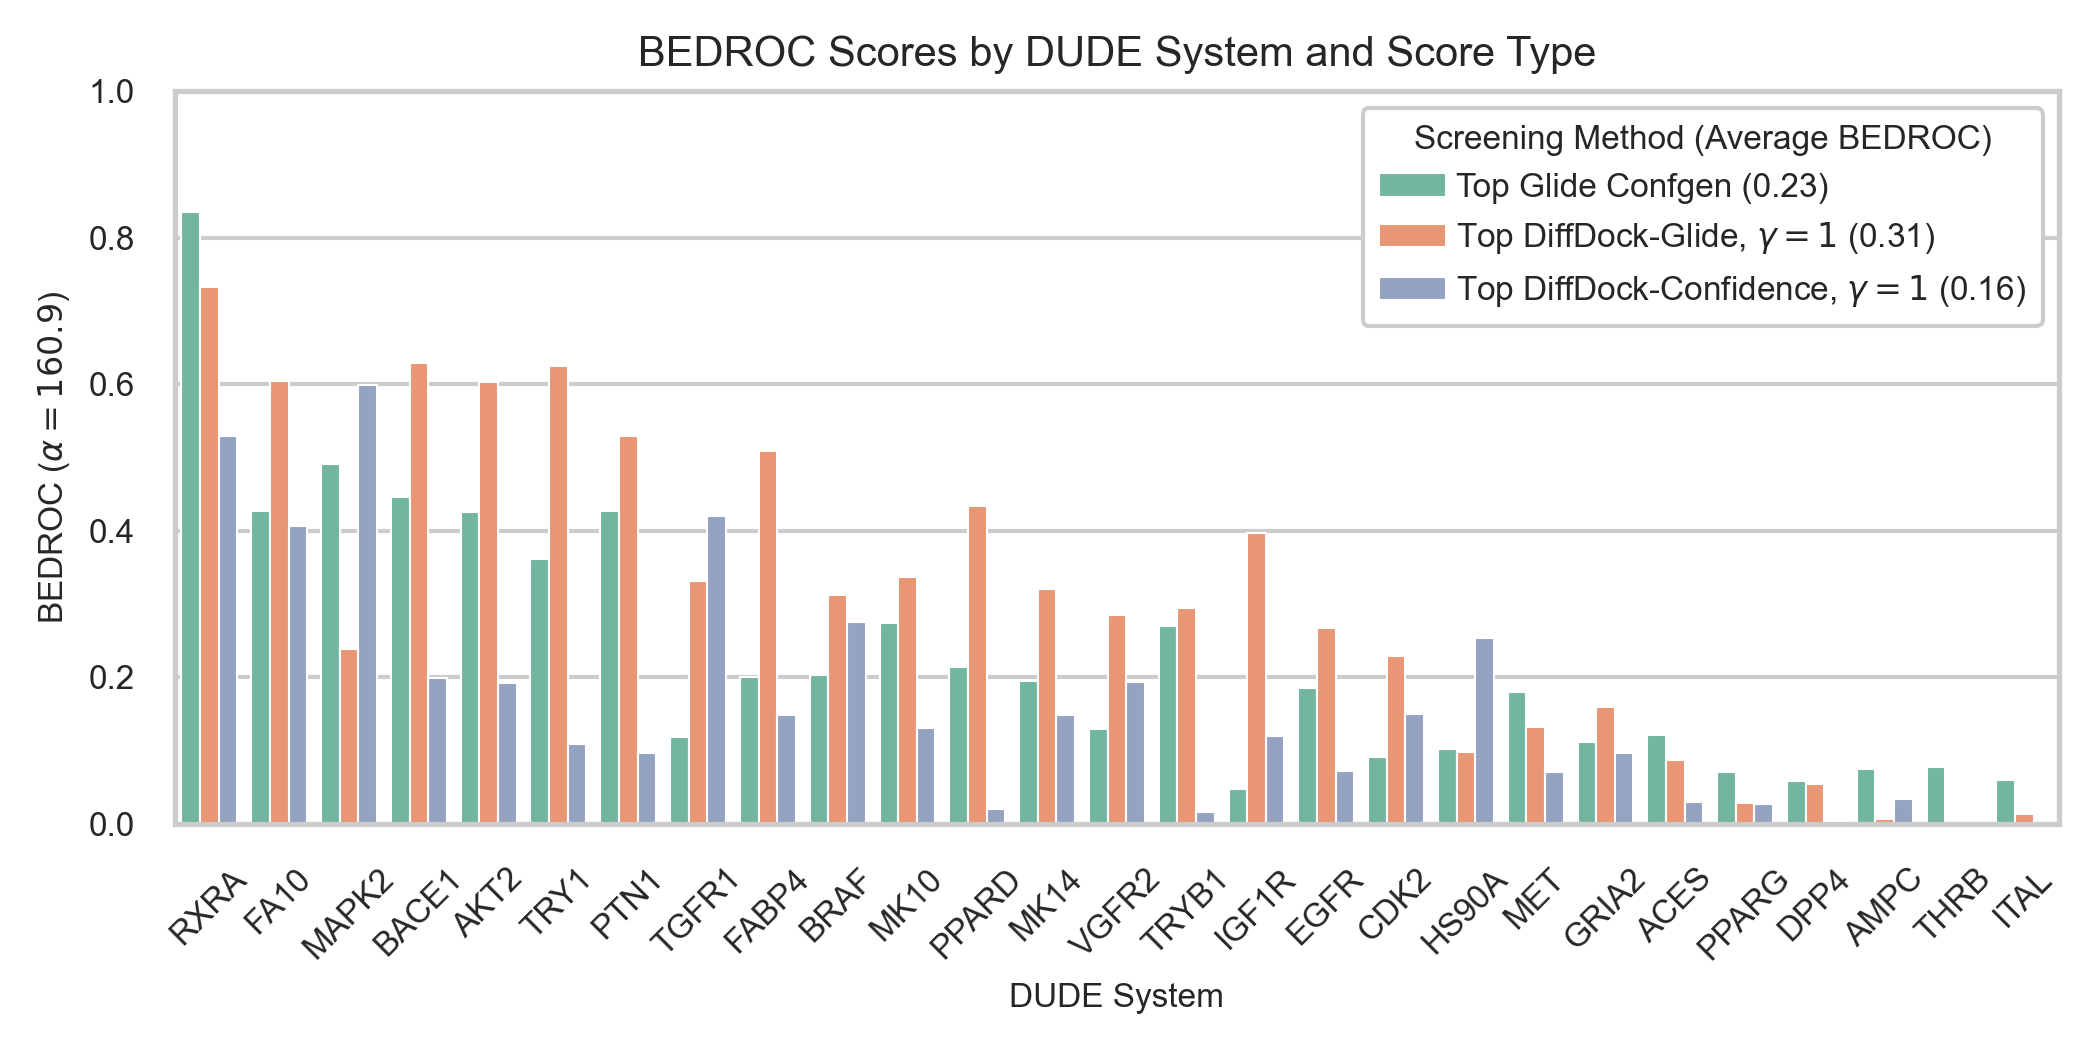
\includegraphics[
   width=\textwidth
   ]{bedroc_calc.png}
   \caption{{\bf Enrichment from virtual screening DUDE compounds against AF2 receptors.} BEDROC enrichments are displayed for the 27 DUDE test systems. Five poses were sampled per compounds by DiffDock-Glide. Compounds are ranked according to three scores for the BEDROC calculation: the top Glide score (blue) and the top (orange) and mean (green) DiffDock-Glide score of the five sampled poses. Systems are sorted according to descending Glide Confgen score.}
   \label{fig:bedroc}%
\end{figure*}

In-silico hit identification utilizes computational methods to discover potential drug candidates, or "hits," from chemical libraries. Both ligand-based and structure-based methods, such as molecular docking, are recognized approaches that screen large chemical libraries to select compounds likely to bind to a target protein structure. Ligand-based methods identify hit compounds by comparing their features to known active ligands, which limits screening of compounds to similar chemical structures. Alternatively, molecular docking tools operate on protein structural information to predict the binding interactions of potential compounds, and do not require feature similarity across ligands. Using molecular docking expands hit identification into unexplored chemical spaces, by not subjecting to limited compound diversity.

A successful virtual screening campaign effectively prioritizes active compounds (ligands with the most favorable energy scores) over inactive compounds, to show early enrichment of actives in the rank ordering. In virtual screening, molecular docking is used as a preliminary filter to eliminate many non-binders and reduce the number of experimental binding calculations of remaining potentially active ligands. Structure based virtual screening relies on an experimental crystallized or computationally-derived protein model. If a \textit{holo} model is available for a specific protein target i.e. a 3-dimensional co-crystallized structure of a target protein bound to its native ligand or co-factor, it offers insight in the protein's active form -- where the binding of a ligand induces conformational changes, and potentially explains the mechanism of action. Therefore, any information related to the binding pocket should be utilized in structure-based virtual screening in order to achieve intended functional mechanisms. 

% [Boltzmann-enhanced discrimination of receiver operating characteristic] 

Deep learning docking tools like DiffDock have gained traction for their ability to blindly dock ligands by predicting both the binding site and binding mode of protein-ligand complexes without prior knowledge of the binding location. However DiffDock's performance in binding site prediction reveals a bias towards sites present in the complexes from the PBD Bind 2020 General Set. As noted in the DockGen benchmark \cite{corso2024dockgen} DiffDock poorly predicts binding poses on unseen binding pockets. For targets deemed "undruggable" at their orthosteric or active sites (where drugs typically bind), an alternative strategy is to design molecules targeting allosteric regions or other areas on the protein's topology. In such cases, constraining the search space is necessary for site-specific target enablement in virtual screening.

Glide is a rigid receptor docking tool that relies on high-quality physically-accurate receptor structures when searching for the lowest-scoring binding pose. On the other hand, DiffDock infers binding poses solely based on the $\alpha$-carbon coordinates, rendering it blind to incorrect sidechain placements. These attributes suggest that DiffDock-Glide should perform well when screening against low-quality receptor structures. We test our hypothesis by screening active and decoy compounds in the DUDE dataset against receptor structures generated by AF2 using Glide and the hybrid DiffDock-Glide algorithm. Since DiffDock-Glide probabilistically samples a distribution of poses and scores, we test the top and mean Glide scores of sampled poses.

Figure \ref{fig:bedroc} reports the BEDROC\cite{truchon2007bedroc} ($\alpha=160.9$) enrichments for the 27 DUDE receptors that do not contain ligands, cofactors, or steric clashes between the {\it holo} ligand and the AF2 structure. Intuitively, a higher BEDROC value indicates a more correct ranking of actives over decoys, with $\alpha=160.9$ non-linearly emphasizing the top 1\% of rankings, i.e. emphasizing early enrichment. For each DUDE system five poses were sampled, minimized, and scored with the same parameters as the docking study in Section \ref{sec:molecular-docking}. 

\jd{@lukas let's add in the unconditional diffdock-glide results from Gary's run}
\lh{Ok. Will add a table w/ Gary's EF1\% values and my EF1\%.}

Both the mean and top DiffDock-Glide scores are capable of producing enrichments rivaling and surpassing Glide Confgen. We further find a high correlation ($r^2=0.98$) between BEDROC enrichments from Glide Confgen and the minimum DiffDock-Glide scores. However, the mean DiffDock-Glide BEDROC values show little correlation with both the Glide Confgen ($r^2=0.28$) and minimum DiffDock-Glide ($r^2=0.36$) enrichments across systems. As such, the mean score serves as an alternative non-redundant ranking metric to the minimum score. Our findings demonstrate that the hybrid DiffDock-Glide algorithm consistently achieves greater early enrichment compared to Glide alone, indicating that DiffDock contributes additional early recognition to virtual screens, provided the receptor structures have high sequence similarity to those in PDBBind General Set v2020.

\section{Outlook}
In this work we have developed a hybrid approach to molecular docking called DiffDock-Glide that mitigates some of the downsides of data-driven approaches to docking. The core idea is to use a data-driven generative model to sample from a learned distribution of binding poses and subsequently relax the sampled poses with a physics-based energy function. 

We benchmark DiffDock-Glide on the PoseBusters dataset and broadly improve on the DiffDock baseline, though our approach still falls short of the performance achieved by Glide Confgen. Our results show that DiffDock-Glide has a weaker dependence on sequence similarity to the training set compared to DiffDock, and that conditioning the generative model on a binding site increases the fraction of crystal-like poses selected. Still, the primary limitation of DiffDock-Glide is (1) sampling crystal-like poses and (2) selecting a crystal-like pose from the sampled distribution. We find that neither the confidence model ranking nor the Glide score of the relaxed poses are able to reliably select the closest generated pose to the crystal structure, indicating the need for more discriminative energy functions or pose refinement beyond energy minimization.

Next we explore using DiffDock-Glide for virtual screening. We use Glide Confgen and DiffDock-Glide to screen active and decoy compounds from the DUDE dataset against 27 AF2-generated target receptor structures and find that the BEDROC enrichments obtained by DiffDock-Glide often exceeds that of Glide Confgen, though all the screened targets except {\it PPARD} are found in DiffDock's training set. We evaluate enrichment based on the top-scoring pose and the mean score among all generated poses finding that both yield increased enrichment over Glide Confgen and have little correlation with one another across systems.

\lh{Recommended use case: cryptic pockets}

\lh{Examine ligand cores in depth for one DUDE target.}



% Remark on how to decide between using the minimum and mean scores. It appears that the mean score produces the best enrichment when Glide performs poorly.

\section{Software and Data}

All Glide calculations were performed using Schrodinger Suite (2023-2 release). We used two datasets to conduct the virtual screening: DUD-E 
(http://dude.docking.org) and the AF2 database (https://alphafold.ebi.ac.uk). The AF2 structures are the same as those in \cite{zhang2023benchmarking}... 
\bibliography{main}
\clearpage


\end{document}